\documentclass{standalone}

\usepackage{tikz}
\usepackage{circuitikz}

\tikzset{block/.style = {draw, fill=white, very thick, rectangle, minimum height=1cm, minimum width=2cm},
         lblock/.style={draw,fill=white,very thick, rectangle, minimum height=3cm, minimum width=1cm},
         sum/.style= {draw, fill=white, very thick, circle, node distance=0.5cm}}

         
\begin{document}
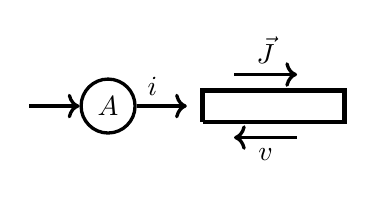
\begin{tikzpicture}[scale=2]
    \node[sum](sum)at(0,0){$A$};
    \draw[->,very thick](-0.5,0)--(sum.180);
    \draw[->, very thick](sum.0)node[above right]{$i$}--(0.5,0);

    \draw[-,ultra thick](0.6,-0.1)--(0.6,0.1)--(1.5,0.1)--(1.5,-0.1)--(0.6,-0.1);
    \draw[->,very thick](0.8,0.2)--(1.2,0.2)node[midway, above]{$\vec{J}$};
    \draw[<-,very thick](0.8,-0.2)--(1.2,-0.2)node[midway, below]{$v$};
\end{tikzpicture}
\end{document}